\subsection{MAPC: Contest and Scenario}
What is the general scenario? Agents on mars trying to find water in a competitive manner against another team. Explain the concept of zones, gaining points, achievements and also how agents differ from each other. Introduce the notion of \emph{zoning} as the process of finding, forming, defending and destroying a zone.
I've put this section first so the later chapters can already rely on the reader knowing what the scenario is about. Furthermore, we can then directly rule out concepts which we are presenting by applying them theoretically onto the scenario/our needs.

\subsection{Agent Programming Concepts}
% I'd actually prefer Subsubsections numbered, without the trailing dot
% and with real section padding. But that's part of the template, so…
\subsubsection{BDI.}
\subsubsection[Formal Methods.]{Formal Methods.$^\diamond$}
As was mentioned in ~\autoref{fun:BDI}, usage of BDI agents brings up several challenges.
One of the important challenges of multi-agent systems is to make sure that the agent will not behave in an unacceptable or undesirable way.
Agents may act in complex production environments, where failure of a single agent may cause serious losses.
Formal methods have been used in computer science as a basis to solve correctness challenges.
They represent agents as a high-level abstractions in complex systems.
Such a representation can lead to simpler techniques for design and development.

There are two roles of formal methods in distributed artificial intelligence that are often referred to.
Firstly, with respect to precise specifications they help in debugging specifications and in validation of system implementations.
Abstracting from specific implementation leads to better understanding of the design of the system being developed.
Secondly, in the long run formal methods help in developing a clearer understanding of problems and their solutions. \cite{Singh_99}

To formalise the concepts of multi-agent systems different types of logics are used, such as propositional, modal, temporal and dynamic logics.
In the following several paragraphs these logics, their properties and introduced operators will be briefly discussed.
Describing the details of interpretations and models of each individual logic is not the purpose of this report and is left out for further reading.

Propositional logic is the simplest logic and serves as the basis for logics discussed further in this section.
It is used to represent factual information and in our case is most suitable to model the agents' environment.
Formulas in this logic language consist of atomic propositions (represinting known facts about the world) and truth-functional connectives: $\land,\lor,\neg,\rightarrow$ which denote \enquote{and}, \enquote{or}, \enquote{not} and \enquote{implies}, respectively~\cite{Enderton_72}.

Modal logic extends propositional logic by introducing two different modes of truth: possibility and necessity.
In the study of agents, it is used to give meaning to concepts such as belief and knowledge.
Syntactically, modal operators in modal logic languages are defined as $\Diamond$  for possibility and $\Box$ for necessity.
The semantics of modal logics are traditionally given in terms of sets of so-called \emph{possible worlds}.
A world here can be interpreted as a possible state of affairs or sequence of states of affairs (history).
Different worlds can be related via a binary accessibility relations, which tells us which worlds are within the realm of possibility from the point of view of a given world.
In the sense of the accessibility relation, a condition is assumed \emph{possible} if it is true somewhere in the realm of possibility and it is assumed \emph{necessary} if it is true everywhere in the realm of possibility~ \cite{Saul_63}.

Dynamic logic is also referred to as modal logic of action.
It adds different atomic actions to the logic language.
In our case, atomic actions may be represented as actions that agents can perform directly.
This makes dynamic logic very flexible and useful for distributed artificial intelligence systems.
Necessity and possibility operators of dynamic logic are based upon the kinds of actions available~\cite{Kozen_90}.

Temporal logic is the logic of time.
There are several variations of this logic, such as:
\begin{description}
  \item[Linear] (or \emph{branching}): single course of history or multiple courses of history.
  \item[Discrete] (or \emph{dense}): discrete steps (like natural numbers) or always having intermediate steps (like real numbers).
  \item[Moment-based] (or \emph{period-based}): atoms of time are points or intervals.
\end{description}
We will concentrate on discrete moment-based models with linear past, but consider both linear and branching futures.

Linear temporal logic introduces several important operators. $p\cup q$ is true at a moment $t$ on a path, if and only if $q$ holds at a future moment on the given path and $p$ holds on all moments between $t$ and the selected occurrence of $q$.
$Fp$ means that $p$ holds sometimes in the future on the given path.
$Gp$ means that $p$ always holds in the future on the given path.
$Xp$ means that $p$ holds in the next moment.
$Pq$ means that $q$ held in a past moment~\cite{Singh_99}.

\begin{figure}[h!]
  \caption{An example branching structure of time~\cite{Singh_99}.}
  \centering
  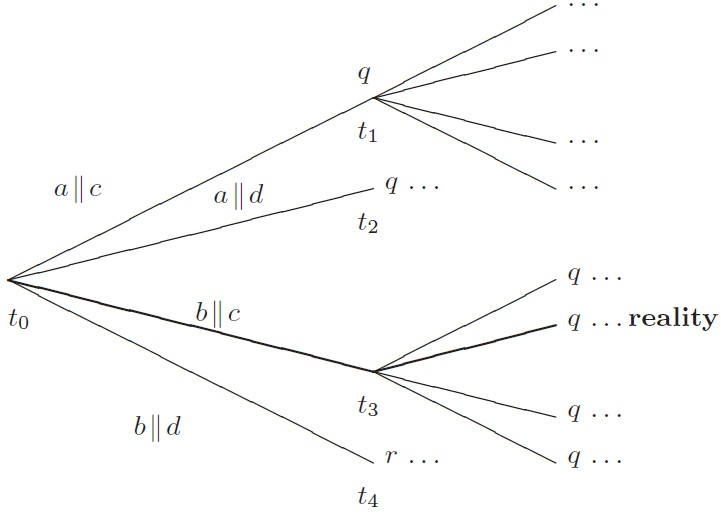
\includegraphics[width=0.6\textwidth]{images/branching_logic.png}
  \label{fig:for_branching_figure}
\end{figure}

Branching temporal and action logic is built on top of both dynamic and linear temporal logics and captures the essential properties of actions and time that are of value in specifying agents.
It also adds several specific branching-time operators.
$A$ denotes \enquote{in all paths at the present moment}.
The present moment here is the moment at which a given formula is evaluated.
$E$ denotes \enquote{in some path at the present moment}.
The reality operator $R$ denotes \enquote{in the real path at the present moment}.
\autoref{fig:for_branching_figure} illustrates the example of branching time for two interacting agents.

For modeling intelligent agents, quite often the BDI concept is used, which was described earlier in this report.
BDI stands for three cognitive specifications of agents: beliefs, desires and intentions.
To model logic of these specifications we will need to introduce several modal operators: $Bel$ for beliefs, $Des$ for desires, $Int$ for intentions and $K_h$ for know-how.
Considering these operators, for example, the mental state of an agent who desires to win the lottery and intends to buy a lottery ticket sometime, but does not believe that he will ever win can be represented by the following formula: $DesAFwin \land IntEFbuy \land \neg BelAFwin$.
For simplification in future we will consider only those desires which are mutually consistent.
Such desires are usually called goals.

It is important to note several important properties of intentions, which should be maintained by all agents~\cite{Singh_92}:
\begin{description}
  \item[Satisfiability] $xIntp\rightarrow EFp$.
    This means that if $p$ is intended by $x$, then it occurs eventually on some path.
    An intention following this condition is assumed to be satisfiable.
  \item[Temporal consistency] $(xIntp \land xIntq)\rightarrow xInt(Fp \land Fq)$.
    This requires that if an agent intends $p$ and intends $q$, then it (implicitly) intends achieving them in some undetermined temporal order: $p$ before $q$, $q$ before $p$, or both simultaneously.
  \item[Persistence does not entail success] $EG((xIntp) \land \neg p)$ is satisfiable.
    This is quite intuitive: just because an agent persists with an intention does not mean that it will succeed.
  \item[Persist while succeeding] This constraint requires that agents desist from revising their intentions as long as they are able to proceed properly.
\end{description}

The concepts introduced above may be used in each of the two roles of formal methods introduced earlier.
The two most commonly used reasoning techniques to decide an agent's actions are theorem proving and model checking.
The first one is more complex in terms of calculations, when the second one is more practical, but it requires additional inputs, though it does not prove to be a problem in several cases.

Considering the practical implementation, the architecture of an abstract BDI-interpreter can be described as follows.
The inputs to the system are called events, and are received via an event queue.
Events can be external or internal in relation to the system.
Based on its current state and input events, the system selects and executes options, corresponding to some plans.
The interpreter continually performs the following: determine available options, deliberate to commit to some options, update the state and execute chosen atomic actions.
After that, it updates the event queue and eliminates the options which have already achieved or are no longer possible.

\todo{Add or leave out a caption for all listings. Currently we are not consistent with that.}
\begin{lstlisting}[caption={An abstract BDI interpreter~\cite{Singh_92}.}]
  BDI-Interpreter
  initialise_state();
  do
    options := option-generator(event-queue, B, G, I);
    selected-options := deliberate(options, B, G, I);
    update-intentions(selected-options, I);
    execute(I);
    get-new-external-events();
    drop-successful-attitudes(B, G, I);
    drop-impossible-attitudes(B, G, I);
  until quit.
\end{lstlisting}

As was mentioned above, options are usually represented by plans.
Plans consist of the name or type, the body usually specified by a plan graph, invocation condition (triggering event), precondition specifying when it may be selected and add list with delete list, specifying which atomic propositions to be believed after successful plan execution.
Intentions in this case may be represented as hierarchically related plans.

Getting back to the algorithm and assuming plans as options, the option generator may look like the following.
Given a set of trigger events from the event queue, the option generator iterates through the plan library and returns those plans whose invocation condition matches the trigger event and whose preconditions are believed by the agent.

\begin{lstlisting}[mathescape, caption={Option generation for BDI interpreter~\cite{Singh_92}.}]
  option-generator(trigger-events, B, G ,I)
  options := {};
  for trigger-event $\in$ trigger-events do
    for plan $\in$ plan-library do
      if matches(invocation(plan, trigger-event) then
        if provable(precondition(plan), B) then
          options := options $\cup$ plan;
  return options.
\end{lstlisting}

Deliberation of options should conform with the execution time constraints, therefore under certain circumstances random choice might be appropriate.
Sometimes lengthy deliberation becomes possible by introducing meta-level plans into the plan library, which form intentions towards some particular plans.

\begin{lstlisting}[mathescape, caption={Option deliberation for BDI interpreter~\cite{Singh_92}.}]
  deliberate(options)
  if length(options) $\leq$ 1 then return options;
  else metalevel-options :=
            option-generator(b-add(option-set(options)));
    selected-options := deliberate(metalevel-options);
    if null(selected-options) then
        return random-choice(options);
    else return selected-options.
\end{lstlisting}

Coordination is one of the core functionalities needed by multi-agent systems.
Especially when different agents act autonomously and have different roles and possible actions.

One of the approaches developed by Singh~\cite{Singh_97} represents each agent as a small skeleton, which includes only the events or transitions made by the agent that are significant for coordination.
The core of the architecture is the idea that agents should have limited knowledge about the designs of other agents.
This limited knowledge is called the significant events of the agent.
There are four main types of events:
\begin{itemize}
  \item flexible, which can be delayed or omitted,
  \item inevitable, which can only be delayed,
  \item immediate, which the agent is willing to perform immediately,
  \item triggerable, which the agent performs based on external events.
\end{itemize}
These events are organised into skeletons that characterise the coordination behavior of agents.
The coordination service is independent of the exact skeletons or events used by agents in a multi-agent system.

To specify coordinations, a variant of the linear-time temporal language with some restrictions is used.
Two temporal operators are introduced for this purpose: $\cdot$, which is the before operator, and $\bigodot$, which is the operator of concatenation of two time traces, the first of which is finite.
Such special logic allows a variety of different relationships to be captured.

Overall, formal methods provide a logic abstraction for multi-agent systems.
They help to find self-consistent models of an agent's behavior.
However, relatively high complexity does not allow these methods to be implemented in real-time systems.
Therefore, the role of formal methods nowadays is limited to debugging, validation and design purposes.

In our project we unfortunately did not apply any formal methods for debugging or validating, mostly because of the limited time for development.


\subsubsection[Negotiation and Argumentation.]{Negotiation and Argumentation.$^\diamond$}
In multi-agent environment, where each agent has its own beliefs, desires and goals, achieving a common goal usually require some sort of cooperation. It most of the cases it can be achieved through communication and negotiation among groups of agents. Often negotiation is supported by some arguments which help to identify which agent is more suitable for completing certain task. Among them could be better position, better resources for completing the task, importance of current goal and so on. Some arguments can be also used to change the intentions of other agents. This could be the arguments like reserving the node to explore or the enemy to attack and many others. Argumentation is essential when agents don't have the full knowledge about other agents or environment. In such cases exchanging information helps to develop the consensus and make cooperative decisions.

To negotiate effectively a BDI agent requires the ability to represent and maintain the model of its own properties, such as beliefs, desires, intentions and goals, reason with other agents' properties and be able to influence other agent's properties \cite{Kraus_98}. These requirements should be supported by the agent programming language we choose for our project. 

As was mentioned above, negotiation is performed through communication. Negotiation messages can be of the following three types: a request, response, or a declaration. A response can take the form of an acceptance or a rejection. Messages can also have several parameters for justification or transmitting negotiation arguments. The arguments are produced independently by each agent using the predefined rules, which will be discussed later in this subchapter. Every agent can send and receive messages. Evaluating a received message is the vital part of negotiation procedure. Only the evaluation process following an argument may change the core agents' beliefs, desires, intentions or goals. 

There are always several ways of modelling agents for negotiation. Agents can be bounded if they do not believe in "false"; omniscient if their beliefs are closed under inferences; knowledgable if  their beliefs are correct; unforgetful if they never forget anything; memoryless if they do not have memory and they cannot reason about past events; non-observer if their beliefs may change only as a result of message evaluation; cooperative if they share the common goal \cite{Kraus_98}. For our project in most of the cases we assumed agent as knowledgable and memoryless - agents remember only about the current round of negotiation and abolish previous round results, when the new round starts. During the zone building process the agents also act as cooperative, since they share the common goal of building a zone.



\subsubsection{Agent Societies.}
\subsection[Agent Programming Languages]{Agent Programming Languages$^\circ$}
An important part of artificial intelligence research deals with autonomous agents acting in environments which are not or only partially known to the agents in the beginning. Allowing agents to reason about their knowledge and interacting with the environment is tackled by different programming methods. This technical report introduces the two logic programming languages GOLOG and FLUX. The basic structure of each language will be shown together with examples to ease understanding. In the first section the situation calculus will be presented. It is a logic formalism GOLOG builds upon. The two subsequent \autoref{fun:apl_golog} and \autoref{fun:apl_flux} cover GOLOG and FLUX respectively. This report closes with a conclusion drawn from the features of GOLOG and FLUX regarding a multi-agent scenario with incomplete knowledge.
--

Why are AS(L) and Jason so awesome that we chose them over the other options? Why didn't we invent our own language or at least our own system/architecture/infrastructure?
% TODO: extend for whole subsection

\subsubsection{Situation Calculus.}\label{fun:apl_sitCalc}
This section gives a short summary of the situation calculus, which was first introduced by McCarthy and Hayes~\cite{mccarthy_philosophical_1969}. The situation calculus is mainly a first-order logic but also uses second order logic to encode a dynamic world \cite{levesque_golog:_1997}. %60
It consists of the three first-order terms: \emph{fluents}, \emph{actions} and \emph{situations} \cite{mccarthy_philosophical_1969,boutilier_decision_2000}. %18+,356
Fluents model properties of the world. Actions may change fluents and hence may modify the world. Every action execution creates a new situation. This is because a situation is a history of actions up to a certain point in time starting from the initial situation $s_0$~\cite{schiffel_reconciling_2006,levesque_golog:_1997}. %289, 60+
There can only be one initial situation as it models the situation before any action has been executed~\cite{pirri_contributions_1999}. %329

Fluents can be evaluated to return a result. As they are situation dependent, the evaluation result may change over time. Fluents are distinguished in \emph{relational fluents} and \emph{functional fluents}~\cite{levesque_golog:_1997}. %3
Relational fluents can hold in situations. Their evaluation hence may return either true or false~\cite{boutilier_decision_2000}. %356
An example is given in \autoref{f_hasCoffee}. It expresses whether or not the agent $p$ has a coffee in situation $s$.
\begin{equation}\label{f_hasCoffee}
  \textit{hasCoffee}(p,s)
\end{equation}
Functional fluents return values instead~\cite{levesque_golog:_1997}. %3
As an example, a fluent $\textit{location}(p,s)$ may return some coordinates $(x,y)$ This then expresses the agent $p$'s location in situation $s$.

Actions also depend on situations. The reason for this is that certain actions may only be executed when specific fluents hold. As fluents are only modified by actions, their result can be determined by the history of action executions contained in the current situation. Describing when an action is executable is done by \emph{action precondition axioms}~\cite{lin_state_1994}. %655+
This is expressed by the predicate $\textit{Poss}(a,s)$ with $a$ being an action. As a recurring example, let us think of the ability to pour an agent $p$ coffee. This must only be possible when $p$ does not already have coffee. \autoref{a_possPourCoffee} illustrates how this can be formalised.
\begin{equation}\label{a_possPourCoffee}
  \textit{Poss}(\textit{pourCoffee}(p),s) \Leftrightarrow \neg \textit{hasCoffee}(p,s)
\end{equation}

As mentioned before, the execution of any action must alter the situation: $\textit{do}(a,s) \rightarrow s'$. Its effects on fluents are described by \emph{action effect axioms}. \autoref{a_effectPourCoffee} shows how pouring a coffee to $p$ will result in $p$ having coffee afterwards.
\begin{equation}\label{a_effectPourCoffee}
  \textit{Poss}(\textit{pourCoffee}(p),s) \rightarrow \textit{hasCoffee}\big(p,\textit{do}(\textit{pourCoffee}(p),s)\big)
\end{equation}
In \autoref{a_effectPourCoffee}, it is unclear whether other fluents are affected by the action execution. For example, reasoning about $location(p,s')$ would not be possible with $\textit{do}(\textit{pourCoffee}(p,s)) \rightarrow s'$. This is called the \emph{frame problem} (cf. Hayes~\cite{hayes_frame_1971}). %224
Defining for every fluent how every action does or does not affect it is only a theoretical solution. The reason for that is that the resulting complexity of $\mathcal{O}(A*F)$ would be too high even in most small worlds. A feasible solution to this problem was proposed by Reiter~\cite{reiter_frame_1991}. His approach was to define every effect of all actions only once. Thus, Reiter reduced the complexity to $\mathcal{O}(A*E)$. This solution is known as the \emph{successor state axiom} and is shown in \autoref{sucStateAxiom}.
\begin{equation}\label{sucStateAxiom}
  \mathit{Poss}(a,s)\rightarrow \big[\mathit{F}(\mathit{do}(a,s)) \Leftrightarrow\gamma_\mathit{F}^+(a,s)\vee\mathit{F}(s)\wedge\neg\gamma_\mathit{F}^-(a,s)\big]
\end{equation}
$\mathit{F}(\mathit{do}(a,s))$ means that the fluent $F$ will be true after executing the action $a$. The first part of the disjunction is $\gamma_\mathit{F}^+(a,s)$ and expresses that the action made the fluent true. $\mathit{F}(s)\wedge\neg\gamma_\mathit{F}^-(a,s)$ as the second part expresses that the fluent had been true before and the action had no influence on it. For a reasonable example, there needs to be a second action which does not influence the fluent given in \autoref{f_hasCoffee}. Therefore, the $sing(s)$ action will be introduced which has no effect on any fluents and can be executed anytime as shown in \autoref{a_possSing}.
\begin{equation}\label{a_possSing}
  \mathit{Poss}(\mathit{sing}, s) \Leftrightarrow \top
\end{equation}
Given \autoref{f_hasCoffee}, \ref{a_possPourCoffee}, \ref{a_effectPourCoffee} and \ref{a_possSing} an example can be compiled as done in \autoref{a_sucStateAxiom}:
\begin{equation}\label{a_sucStateAxiom}
  \begin{split}
    \mathrm{Poss}(a,s)\rightarrow \big[&\mathrm{hasCoffee}(p,\mathrm{do}(a,s))
\\    &\Leftrightarrow [a=\mathrm{pourCoffee}(p)]
\\    &\vee\ [\mathrm{hasCoffee}(p,s) \wedge a\neq \mathrm{pourCoffee}(p)]\big]
  \end{split}
\end{equation}
\autoref{a_sucStateAxiom} then formalises that an agent $p$ may only have coffee if it was poured coffee or if it already had coffee and the action was not to pour $p$ a coffee.


\subsubsection{GOLOG.}\label{fun:apl_golog}
This section gives a summary of the logic programming language GOLOG. Moreover, its problems in context of the Mars-scenario are shown. If not further specified, all information except for the examples is taken from Levesque et~al.~\cite{levesque_golog:_1997} who introduced the language. GOLOG builds on the situation calculus. To allow high-level programming, the language adds complex actions like loops, conditions, tests and non-deterministic elements. As an example, a GOLOG program should have a robot pouring other agents coffee until everybody does have coffee. After that, the robot should sing and terminate. Such a program would reuse the fluent of \autoref{f_hasCoffee}, the action precondition axioms of \autoref{a_possPourCoffee} and \ref{a_possSing}, the successor state axiom of \autoref{a_sucStateAxiom} and extend them with the two procedures given in \autoref{p_main} and \ref{p_pourSOCoffee}:
\begin{equation}\label{p_main}
  \begin{split}
    \textbf{proc}\ \texttt{main}\ [&\textbf{while}\ (\exists p) \neg\textit{hasCoffee}(p) \\
    &\textbf{do}\ \texttt{pourSOCoffee}(p)\ \textbf{endWhile}]; \\
    \textit{sing}&\ \textbf{endProc}.
  \end{split}
\end{equation}
\begin{equation}\label{p_pourSOCoffee}
  \begin{split}
    \textbf{proc}\ \texttt{pourSOCoffee}\ (\boldsymbol{\pi} p)\ [ &\neg\textit{hasCoffee}(p)\textbf{?}; \\
    &\textit{pourCoffee}(p)]\ \textbf{endProc}.
  \end{split}
\end{equation}
\autoref{p_main} shows the procedure which can be seen as the main method. It loops as long as there exist agents without coffee and tells the robot to pour some agent coffee which is lacking coffee. In the end, the robot sings. \autoref{p_pourSOCoffee} allows the robot to non-deterministically choose an agent $p$ to pour coffee by using the $\pi$-operator. The $?$-operator is similar to the \texttt{if}-operator in other programming languages like Java. Due to the non-determinsmic operator, there can be two different resulting situations as shown in \autoref{ex_situations} with the initial configuration given in \autoref{ex_gologConfiguration}:
\begin{equation}\label{ex_gologConfiguration}
  \neg\textit{hasCoffee}(p,s_0) \Leftrightarrow p=\textrm{Jane} \vee p=\textrm{John}.
\end{equation}
\begin{equation}\label{ex_situations}
  \begin{split}
    s=\textit{do}\Big(\textit{sing},\textit{do}\big(&\textit{pourCoffee}(\textrm{Jane}),
      \textit{do}(\textit{pourCoffee}(\textrm{John}),s_0)\big)\Big),
\\  s=\textit{do}\Big(\textit{sing},\textit{do}\big(&\textit{pourCoffee}(\textrm{John}),
      \textit{do}(\textit{pourCoffee}(\textrm{Jane}),s_0)\big)\Big)
  \end{split}
\end{equation}

% TODO: I know splitting up by every point looks like shit. But not doing so makes it harder to read. I'm open for suggestions!
Levesque et~al.~\cite{levesque_golog:_1997} highlight multiple problems with GOLOG. Problems which are relevant when considering to apply GOLOG on the Mars-scneario, are given in this part.
One problem is that complete knowledge is assumed in the initial situation. This is not the case for the Mars-scenario and scenarios with unknown worlds that get explored by agents in general.

The second problem is that GOLOG does not offer a simple solution for sensing actions and reactions of agents on sensed actions. Sensing actions are actions by agents that may not modify fluents but the internal knowledge of agents by detecting some properties in the world \cite{thielscher_flux:_2005}. This can be seen as a side-effect of GOLOG not being developed for unknown worlds. Again, this would be a feature which is needed for the Mars-scenario.

A third problem is that exogenous actions cannot be handled. Exogenous actions are actions outside of the agent's control. In the Mars-scenario, this e.g. could be the loss of an agent's health due to an enemy agent attacking it.

Thielscher~\cite{thielscher_flux:_2005} highlights a fourth problem. It arises from GOLOG being \emph{regression-based}. This means that deciding whether an action is executable is only possible after looking at all previous actions and how they might have affected the world. As a result, reasoning takes exponentially longer over time and hence GOLOG does not scale. Due to these problems, GOLOG is unsuitable for a multiple agent-based scenario like the Mars-scenario without considerable modifications and extensions.


% Define a listing style for FLUX code
\lstdefinestyle{flux} { % TODO: I think this must be defined before the beginning of the document to work.
  frame=L,
  xleftmargin=\parindent,
  basicstyle=\footnotesize\ttfamily,
  breakatwhitespace=true,
  numbers=left,
  escapechar=\%,
  numberstyle=\tiny,
  numberblanklines=false,
  captionpos=b,
  emph={perform, poss, state\_update, main\_loop, init},
  emphstyle=\textbf,
}
%
\lstset{style=flux} % activate flux syntax highlighting in listings
\subsubsection[FLUX.]{FLUX.$^\circ$}\label{fun:apl_flux}
This section gives a summary of the logic programming language FLUX which offers solutions to the earlier shown problems of GOLOG.
Except for the examples and if not specified otherwise, the information of this section is taken from Thielscher~\cite{thielscher_flux:_2005} who first introduced FLUX.
This is done by using the \emph{fluent calculus} instead of the situation calculus.
Both are similar but the fluent calculus adds \emph{states}.
A state $z$ is a set of fluents $f_1,\dotsc,f_n$.
In FLUX, it is denoted as $z = f_1 \circ\dotsc\circ f_n$.
In every situation there exists exactly one state with which the current properties of the world are being described.
Yet, the world can be in the same state in multiple situations.
FLUX uses \emph{knowledge states} for representing agent knowledge.
These are denoted through $\textit{KState}(s,z)$ meaning that an agent knows that $z$ holds in $s$.
Knowledge states can be incomplete as opposed to knowledge in GOLOG.

The frame problem in the fluent calculus is solved through \emph{state update axioms} as described by Thielscher~\cite{thielscher_situation_1999}.
The axioms define the effects of an action as the difference between the state before and after the action.
This is modelled with $\vartheta^-$ for negative and $\vartheta^+$ for positive effects.
Both are simply macros for finite states.
Due to using states, reasoning is linear in the size of the state representation.
That is, after every action execution, the world represented by its fluent is processed.
This is called being \emph{progression-based}.
Therefore, FLUX can outperform GOLOG as determining whether a property currently holds is only a matter of looking it up in the state.
With GOLOG however, the property must be traced back to the initial situation by looking at all action executions and their effects. %\cite{thielscher_flux:_2005}

Disjunctive and negative state knowledge is modelled through constraints.
FLUX uses a constraint solver to simplify these constraints until they are solvable.
This is done by using \emph{constraint handling rules} introduced by Frühwirth~\cite{fruhwirth_theory_1998}.
Their general form is shown in \autoref{chr}.
It consists of one or multiple heads $H_m$, zero or more guards $G_k$ and one or multiple bodies $B_n$.
The general mechanism is that if the guard can be derived, parts of the constraint matching the head will be replaced by the body and hence get simplified.
\begin{equation}\label{chr}
  H_1,\ldots,H_m\Leftrightarrow G_1,\ldots,G_k \mid B_1,\ldots,B_n
\end{equation}

A FLUX program can be separated into three main parts with the constraint solver building the kernel which is the foundation of a FLUX program.
The domain encodings are built on top of this.
Included are the initial knowledge state(s), domain constraints, as well as the action precondition and state update axioms.
The final part of a FLUX program is the programmer defined intended agent behaviour called strategy.
As a trivial example program, the previous example implemented in GOLOG will be transferred into FLUX.
This is done by using the logic programming language Prolog in which FLUX is typically implemented~(cf. \cite{thielscher_reasoning_2006,martin_addressing_2001}). % xi, 1085+, 297
The example features the domain encodings as well as the strategy.
\begin{lstlisting}[caption={Defintion of the \texttt{sing}-action.}, label=lst_sing]
  perform(sing, []).
  poss(sing, Z) :- all_holds(hasCoffee(_), Z).%\label{l_possSing}%
  state_update(Z, sing, Z, []).%\label{l_supSing}%
\end{lstlisting}
\autoref{lst_sing} shows the definition of the \texttt{sing}-action.
Empty arrays denoted by \texttt{[]} could be replaced by sensed information.
They would then effect the outcome of the methods.
As this is a trivial example, no sensed information is assumed.
\autoref{l_possSing} is the precondition that singing is only possible in a state where every agent has coffee.
As singing should not alter any fluents, the state \texttt{Z} in \autoref{l_supSing} is not modified and returned again as \texttt{Z}.
\begin{lstlisting}[firstnumber=4, caption={Definition of the \texttt{pourCoffee}-action}, label=lst_pourCoffee]
  perform(pourCoffee(P), []).
  poss(pourCoffee(P), Z) :-
       member(P,[jane,john]),%\label{l_memberP}%
       not_holds(hasCoffee(P), Z).
  state_update(Z1, pourCoffee(P), Z2, []) :-
       update(Z1, [hasCoffee(P)], [], Z2).%\label{l_updateZ}%
\end{lstlisting}
The \texttt{pourCoffee}-action is defined similarly in \autoref{lst_pourCoffee}.
\autoref{l_memberP} ensures that Prolog will only look for agents that actually exist instead of iterating over memory addresses.
The action must modify the state by adding \texttt{hasCoffee(P)} to the state as it is done in \autoref{l_updateZ}.
The array after it corresponds to $\vartheta^-$.
It is empty in this case as no fluents are removed.
\begin{lstlisting}[firstnumber=10, caption={Main method which either tells the robot to sing or to pour coffee.}, label=lst_main]
  main_loop(Z) :-
    poss(sing, Z)
      -> execute(sing, Z, Z);
    poss(pourCoffee(P), Z)
      -> execute(pourCoffee(P), Z, Z1),
         main_loop(Z1);
    false.%\label{l_false}%
\end{lstlisting}
\autoref{lst_main} models the main method and thus is similar to \autoref{p_main}.
When singing is possible, the robot will do so and terminate.
Else, it will pour someone a coffee and call the main loop again.
\autoref{l_false} ensures that Prolog will return the false-value \texttt{No} if neither of the both actions get triggered at some point.
\begin{lstlisting}[firstnumber=17, caption={Initial configuration.}, label=lst_init]
  init(Z0) :-
         not_holds(hasCoffee(jane), Z0),
         not_holds(hasCoffee(john), Z0).
\end{lstlisting}
The initial configuration in \autoref{lst_init} is comparable to \autoref{ex_gologConfiguration} but due to Prolog interpreting from top to bottom, the result will be \texttt{Z = [hasCoffee(john), hasCoffee(jane)]}.

Schiffel and Thielscher~\cite{schiffel_multi-agent_2007} successfully applied FLUX to the gold mining domain.
It is a scenario where multiple agents with different roles work together on mining gold in an unknown terrain~\cite{schiffel_multi-agent_2007}.
The requirements for solving the problems arising from this scenario are comparable to those appearing in the Mars-scenario.
Given the former short presentation and this knowledge, it can be said that FLUX could be applied to the Mars-scenario.


\subsubsection{Jadex.}

\subsubsection[AgentSpeak(L)]{AgentSpeak(L)$^{\circ,\dagger}$}\label{fun:apl_asl}
This section provides an overview of the general concepts of the logic programming language AgentSpeak(L).
The language was developed by Rao~\cite{anand_AgentSpeak_1996}.
Except for the examples, this section takes its information from the cited paper.
The idea behind AgentSpeak(L) was to make the theoretic concept of BDI agents usable in practical scenarios. % 44

The main language constructs are \emph{beliefs}, \emph{goals} and \emph{plans}.
Beliefs represent information that an agent has about its environment.
A belief \texttt{hasCoffee(p)} for example denotes that an agent knows that the person \texttt{p} has coffee.
In AgentSpeak(L), variables are indicated by using a capital first letter whereas terms with a lower-case initial letter are constants. % 45
\begin{lstlisting}[caption={Initial beliefs.}, label=lst:asl_initBeliefs]
  ~hasCoffee(jane).
  ~hasCoffee(john).
\end{lstlisting}
\autoref{lst:asl_initBeliefs} shows the initial beliefs of an agent in the example we just introduced.
The tilde ($\sim$) expresses that the agent knows that neither \texttt{john} nor \texttt{jane} has coffee.
At any given time, the sum of all current beliefs of an agent are called its \emph{belief base}~\cite{bordini_jason_2005}. % p.8

Goals can be divided into \emph{achievement goals} and \emph{test goals}.
The first expresses the wish of an agent to reach a state where a belief holds where the second tests whether a belief holds in the current state.
Beliefs hold when the agent knows they are true or when the variables can be bound to at least one known configuration.
For example, a given achievement goal \texttt{!hasCoffee(p)} means that an agent wants to achieve that person \texttt{p} has coffee.
Similarly, \texttt{?hasCoffee(p)} expresses that an agent tests whether \texttt{p} has coffee.
Hence, this expression will evaluate to true or false depending on the agent's knowledge.
Achievement goals are comparable to desires. % 45
\autoref{lst:asl_initGoal} shows the initial achievement goal which express that the agent wants to have served everyone coffee.
\begin{lstlisting}[firstnumber=3, caption={Initial goal.}, label=lst:asl_initGoal]
  !servedCoffee.
\end{lstlisting}

\emph{Events} are introduced to allow agents to react on changes in their own knowledge or the world.
They can be distinguished into the addition and removal of beliefs or goals.
Additions are denoted by a plus (+) and removals by using a minus (-) sign in front of the goal or belief:
\begin{itemize}
  \item \texttt{+hasCoffee(p)}: an agent is informed that \texttt{p} now has coffee.
  \item \texttt{-hasCoffee(p)}: an agent is informed that \texttt{p} no longer has coffee.
  \item \texttt{+!hasCoffee(p)}: an agent is informed that it wants \texttt{p} to have coffee.
  \item \texttt{-!hasCoffee(p)}: an agent is informed that it no longer wants \texttt{p} to have coffee.
  \item \texttt{+?hasCoffee(p)}: an agent is informed that it should test for the belief.
  \item \texttt{-?hasCoffee(p)}: an agent is informed that it no longer needs to test for the belief.
\end{itemize}
In order to handle new events, an agent will look for a matching plan.

Plans can be seen as programmer-defined agent instructions.
They lead to the execution of actions or the splitting of goals into additional goals.
Plans which an agent wants to execute, are similar to intentions for BDI agents.
They are stored as a set of intentions.
The set of plans generally known to an agent is called the \emph{plan library}~\cite{bordini_jason_2005}.
A plan is triggered by events and is context-sensitive.
This means that the execution of a plan can be restricted to states in where certain beliefs exist.
\autoref{lst:asl_sing} illustrates this by showing when the \texttt{sing} action is being executed.
\autoref{l:asl_trigger} is the triggering event of the plan.
In this case, an agent will consider executing this plan, when it notices that someone is poured coffee.
Hence, this plan is called a \emph{relevant plan}.
The underscore (\texttt{\_}) denotes an anonymous variable similar to its use in Prolog.
Its meaning is that it will match any term.
\autoref{l:asl_context} is the plan's context.
The plan is called an \emph{applicable plan} if the context's beliefs are all known to the agent.
In this particular case, the agent must know that there is no person without coffee indicated by the use of the tilde.
Lastly, \autoref{l:asl_body} contains the body of the plan.
Here, the agent should achieve the goal \texttt{sing}.
This will trigger a new event which calls the plan in \autoref{l:asl_sing}.
As its context is empty, the plan can be executed immediately and evaluates to true as there is no body.
\autoref{l:asl_loop} expresses how the event of someone being poured coffee should be alternatively handled.
As AgentSpeak(L) is interpreted from top to bottom, it will only be seen as an applicable plan, if the former relevant plan did not trigger.
Therefore, if the agent knew that there was still someone left without coffee, it will want to achieve the \texttt{servedCoffee} goal again.
% TODO?: explain that this is a better example and hence we first deal with it instead of servedCoffee
\begin{lstlisting}[firstnumber=4, caption={Events for handling someone being poured a coffee as well as the \texttt{sing} plan.}, label=lst:asl_sing]
  +hasCoffee(_):%\label{l:asl_trigger}%
      ~hasCoffee(_)%\label{l:asl_context}%
      <- !sing.%\label{l:asl_body}%
  +hasCoffee(_)%\label{l:asl_loop}%
      <- !servedCoffee.
  +!sing.%\label{l:asl_sing}%
\end{lstlisting}
% We assume that the implementation of AgentSpeak(L) does not do anything if there is no applicable plan for an event. In \autoref{lst:asl_sing} this would be equal to adding a plan for \texttt{hasCoffee(\_)} without context or body. Given this assumption, the \texttt{pourCoffee}-action is then defined as shown in \autoref{lst:asl_pourCoffee}. \autoref{l:asl_pourCoffee} uses a shortcut operator which extends to \texttt{-hasCoffee(\_); +hasCoffee(X)} \cite{bordini_programming_2007}. % 53
\autoref{lst:asl_serve} contains the plan for serving coffee.
It uses a test goal to pick someone without a coffee as shown in \autoref{l:asl_thirsty}.
The person will be bound to the variable \texttt{X}.
After that, an achievement goal is added to the agent's set of intentions to pour \texttt{X} coffee.
The plan does not feature any context as this minimal example ensures that the goal \texttt{!servedCoffee} will only exist when there actually is a person without coffee.
\begin{lstlisting}[firstnumber=10, caption={Definition of the \texttt{servedCoffee} plan.}, label=lst:asl_serve]
  +!servedCoffee:
      <- ?~hasCoffee(X);%\label{l:asl_thirsty}%
         !pourCoffee(X).%\label{l:asl_pour}%
\end{lstlisting}
\autoref{lst:asl_pour} shows a plan which states that if an agent receives an event to achieve the goal \texttt{!pourCoffee} for some person \texttt{X}, it will pour coffee for \texttt{X}.
Additionally, the knowledge about \texttt{X} not having any coffee is removed in \autoref{l:asl_coffeeless}.
\begin{lstlisting}[firstnumber=14, caption={Definition of the \texttt{pourCoffee} plan.}, label=lst:asl_pour]
  +!pourCoffee(X)
      <- +hasCoffee(X);
         -~hasCoffee(X).%\label{l:asl_coffeeless}%
\end{lstlisting}

As shown, AgentSpeak(L) is another logic programming language for agent programming.
It was specifically designed for developing BDI-agents.
In the next section, an interpreter for this language will be given, which further extends it.


\subsubsection[Jason]{Jason$^\circ$}\label{fun:apl_jason}
This section gives a quick overview of Jason, which is an interpreter for AgentSpeak(L).
All information if not marked differently is taken from Bordini et al.~\cite{bordini_jason_2005}.
Besides being an interpreter, Jason extends AgentSpeak(L) by several concepts.
The most important ones will be discussed in this section.

With Jason, terms can represent more than a constant or a variable.
They can be strings, integer or floating point numbers or lists of terms.
Therefore, more complex programmatic operations and arithmetic expressions are possible with Jason.
Furthermore, Jason introduces annotations.
With these annotations, metadata can be added to triggering events and beliefs.
This metadata can be accessed programmatically.
\autoref{lst:jason_annotations} shows the earlier used initial beliefs with added annotations.
The \texttt{source} annotation is the only one with its meaning predefined by Jason.
It expresses the source of the information.
If an agent determined something itself, the \texttt{source} is \texttt{self}.
Did the agent receive the information as a perception of the environment, then the \texttt{source} will be \texttt{percept}.
The source can also be a constant identifying a different agent if that agent is the source of this information.
With the example given in \autoref{lst:jason_annotations}, an achievement goal \texttt{?\~{}hasCoffee(X)[reliability(Y)]} will bind \texttt{X} to \texttt{john} and \texttt{Y} to \texttt{0.3}.
The \texttt{reliability} has no further meaning unless the value bound to \texttt{Y} is used later.
\begin{lstlisting}[caption={Annotation of beliefs in Jason.}, label=lst:jason_annotations]
  ~hasCoffee(jane)[source(self)].
  ~hasCoffee(john)[source(percept), reliability(0.3)].
\end{lstlisting}

Another concept added to AgentSpeak(L) by Jason is called \emph{internal actions}.
It was first introduced and implemented by Bordini et al.~\cite{bordini_agentspeak_2002}.
Most characteristic for these actions is that they do not affect the environment in which the agents are located in.
This means they have no effect on the external world but only on the internal states of the agents as the name suggests.
Hence, any effects of internal actions occur immediately after the action execution instead of only after the next environment processing cycle.
As a result, internal actions can not only be used within a plan's body but also in its context. % all this information is from p. 1297
Internal actions start with a dot (.) followed by a library identifier, another dot and finally the action name.
Bordini et al.~\cite{bordini_agentspeak_2002} implemented various internal actions which are not identified by any explicitly named library.
These methods reside in the so called \emph{standard library} and omit the library declaration when being called.
An example of this is \texttt{.gte(X,Y)} which returns the truth value of \texttt{X}$\geq$\texttt{Y}.
A realisation of the same function outside the standard library could e.g.\ be called \texttt{.math.gte(X,Y)}.
The standard library is included in Jason.
Furthermore, Jason extends this library by various actions including multiple list operations like sorting or retrieving the minimum.
Developers can write additional internal actions in Java or any other programming language which supports the programming framework Java Native Interface. %11

Arguably, the most important internal action is \texttt{.send}.
This action enables inter-agent communication as initially proposed and implemented by Vierira et al.~\cite{vieira_formal_2007}.
It is structurally based on KQML and FIPA~\cite{fernandez_evaluating_2010}.
A short overview of a FIPA message has been given in \autoref{fun:apl_jadex}.
We pass on presenting the structure of a KQML message here as both are similar and KQML is not further developed~\cite{obrien_fipatowards_1998}.
\begin{lstlisting}[caption={Parameters of the internal action \texttt{.send} and an example.}, label=lst:jason_send]
  .send(Receiver, Illocutionary_force, Message_content).%\label{l:jason_send}%
  .send([agent1, agent2], tell, ~hasCoffee(john)).%\label{l:jason_sendInstance}%
\end{lstlisting}
In \autoref{l:jason_send} of \autoref{lst:jason_send} the structure of the \texttt{.send} action is shown.
\autoref{l:jason_sendInstance} shows example usage of this action.
The \texttt{Receiver} is the identifying name or a list of identifying names for the agent(s) to which the message should be addressed to.
The \texttt{Illocutionary\_force} is a constant that specifies what all recipients should do with the message.
It can be:
\begin{itemize}
  \item \texttt{tell}: add the \texttt{Message\_content} to the recipient's belief base.
  \item \texttt{untell}: remove the \texttt{Message\_content} from the recipient's belief base.
  \item \texttt{achieve}: add the \texttt{Message\_content} as an achievement goal to the recipient.
  \item \texttt{unachieve}: make the recipient remove the achievement goal \texttt{Message\_content}.
  \item \texttt{tellHow}: \texttt{Message\_content} is added to the recipient's plan library.
  \item \texttt{untellHow}: \texttt{Message\_content} is removed from the recipient's plan library.
  \item \texttt{askIf}: asks if \texttt{Message\_content} is in the recipient's belief base.
  \item \texttt{askOne}: asks for the first belief matching \texttt{Message\_content}.
  \item \texttt{askAll}: asks for all beliefs matching \texttt{Message\_content}.
  \item \texttt{askHow}: demand all plans a recipient has that match the triggering event given in the \texttt{Message\_content}.
\end{itemize}
Jason automatically processes the messages as needed when a message arrives at an agent\todo{should we explicitly talk about an agent's inbox? Compare with @adaudrich's mentioning of the inbox!}.
A developer can override Jason's default behaviour if further or different processing is desired.
Jason also automatically adds \texttt{source} annotations.
This allows agents to determine the sender of any received message.

There is special support for defining environments with Jason.
Instead of having to do this in AgentSpeak(L), it can be done in Java.
For doing so, a developer has to extend the \texttt{Environment} class and specify the \texttt{getPercepts(String agentName)} and \texttt{executeAction(String agentName, Term action)} methods.
The first method must return a list of literals restricted to what the agent identified by \texttt{agentName} can perceive.
When the second method is called, the programmer must specify how the given \texttt{action} affects the environment.
It returns a boolean to indicate whether the execution was successful.
Such an action can fail if for example a Repairer agent would try to execute the \texttt{attack} action, which it cannot according to the rules specified for the \mars scenario.
To call the \texttt{executeAction} method from an agent, all it has to do is execute e.g. \texttt{attack}.
Jason will then call \texttt{executeAction(String agentName, Term action)} with the parameters bound to the agent's name and the \texttt{attack} action.
For the MAPC itself, no fully simulated environment is needed.
Instead, it is enough to delegate the actions to the MAPC server and process the server replies by returning the transmitted percepts to the respective agents.
Therefore, percepts do not have to be modelled or modified in the environment developed with Jason itself.

Jason also allows running multi-agent systems over networks in a distributed manner.
Hence, the workload can be distributed over multiple machines.
SACI~\cite{hubner_saci_2000} and JADE are the two fully implemented distributed architectures usable out of the box with Jason \cite{bordini_programming_2007}.
Fernández et al.~\cite{fernandez_evaluating_2010} could not prove the intended performance benefits.
The authors tested both SACI and JADE with Jason where one host would run the environment and the other one the agents.
They increased both the amount of agents as well as the size of the environment.
Fernández et al.~\cite{fernandez_evaluating_2010} saw that with increasing complexity, the system became slower compared to when agents and the environment were run on a single machine.
This was due to the added communication cost between the two hosts although connected by Gigabit Ethernet.
As a result, a distributed infrastructure with Jason is only advisable, if the workload cannot be handled by one host alone.
In our case, replying in time has such an importance that trying to keeping the workload processable by one host alone would be the preferred strategy.

